\section{总结}

\subsection{工作总结}

本作品完成了一套可复用于不同智能体框架的\textbf{运行时安全中间件}。三级级联按规则、本地模型、脱敏外部裁判有序升级，高危命中立即短路，所有路径归约为允许、询问、拒绝、脱敏后允许四值动作；OpenClaw 首个适配将判定接入四个真实执行点，并以助手绑定、确定性脱敏、内容无关审计和失效闭合强制关键安全性质。

\verb|send_email| 劫持在工具执行前被拒绝，记录拦截 1 次、执行 0 次；九个攻击与对照用例均产生预期动作。300 条封印评测整体为英文、中文各 150 条，覆盖九类风险；其中 54 条第一方对抗变换均为英文。P6 以签名和树哈希证明结构完整；P7 回放封印的 provider 响应并重新执行安全引擎与评测器，验证产物级确定性重放，不是 LLM 推理确定性。

\subsection{应用拓展}

统一契约将框架适配与安全策略解耦。其他框架只需映射运行、模型输出、工具执行和消息外送生命周期，即可复用三级级联、四值归约、脱敏与审计能力；图~\ref{fig:cross-framework} 区分已完成的 OpenClaw 路径与可适配入口。

\begin{figure}[htbp]
\centering
\reportFigureLead{OpenClaw 已完成实线接入；其他框架通过虚线适配层复用同一安全核心，不暗示其已完成实测。}
\resizebox{0.98\linewidth}{!}{%
\begin{tikzpicture}[
  font=\small,
  frame/.style={draw=reportSystem, rounded corners=3pt, minimum width=2.55cm,
                minimum height=0.78cm, align=center, fill=reportSystem!10},
  future/.style={frame,dashed,draw=reportMuted,fill=reportCanvas},
  adapter/.style={draw=reportPass, rounded corners=3pt, minimum width=2.8cm,
                  minimum height=0.82cm, align=center, fill=reportPass!12},
  futureadapter/.style={adapter,dashed,draw=reportMuted,fill=reportCanvas},
  core/.style={draw=reportEvidence, rounded corners=3pt, minimum width=4.0cm,
               minimum height=3.65cm, align=center, fill=reportEvidence!12},
  resultbox/.style={draw=reportSystem, rounded corners=2pt, minimum width=3.0cm,
                   minimum height=1.25cm, align=center, fill=reportSystem!12},
  evidence/.style={draw=reportEvidence, dashed, rounded corners=2pt, minimum width=7.8cm,
                   minimum height=0.82cm, align=center, fill=reportEvidence!5},
  a/.style={-{Stealth[length=1.7mm]}, draw=reportSystem, thick}
]
\node[frame] (openclaw) at (0,1.35) {\textbf{OpenClaw}\\已完成接入};
\node[future] (frameworka) at (0,0) {其他智能体框架 A\\可适配入口};
\node[future] (frameworkb) at (0,-1.35) {其他智能体框架 B\\可适配入口};

\node[adapter] (oa) at (3.55,1.35) {OpenClaw 适配层\\四个真实执行点};
\node[futureadapter] (aa) at (3.55,0) {框架 A 适配层\\生命周期映射};
\node[futureadapter] (ba) at (3.55,-1.35) {框架 B 适配层\\生命周期映射};

\node[core] (core) at (7.75,0) {\textbf{共用运行时安全核心}\\[3pt]
  \texttt{SandboxSecurityRequest}\\
  三级级联与高危短路\\
  四值归约与脱敏升级\\
  内容无关审计\\
  \texttt{SandboxSecurityDecision}};
\node[resultbox] (decision) at (12.0,0) {决策映射回框架屏障\\allow / ask / deny / allow\_sanitized};
\node[evidence] (replay) at (7.75,-3.0) {共用 P6/P7 回归基线：哈希锁定夹具、签名收据、封印 provider 响应重放};

\draw[a] (openclaw) -- (oa);
\draw[a,dashed] (frameworka) -- (aa);
\draw[a,dashed] (frameworkb) -- (ba);
\draw[a] (oa.east) -- (core.west |- oa.east);
\draw[a,dashed] (aa.east) -- (core.west |- aa.east);
\draw[a,dashed] (ba.east) -- (core.west |- ba.east);
\draw[a] (core) -- (decision);
\draw[a,dashed] (core.south) -- (replay.north);
\end{tikzpicture}%
}
\caption{跨框架复用与接入拓扑。实线表示已完成的 OpenClaw 路径，虚线表示其他框架需实现的生命周期适配；三级级联、四值决策、脱敏、审计和 P6/P7 回归基线由安全核心统一复用。}
\label{fig:cross-framework}
\end{figure}

\clearpage
\begin{center}
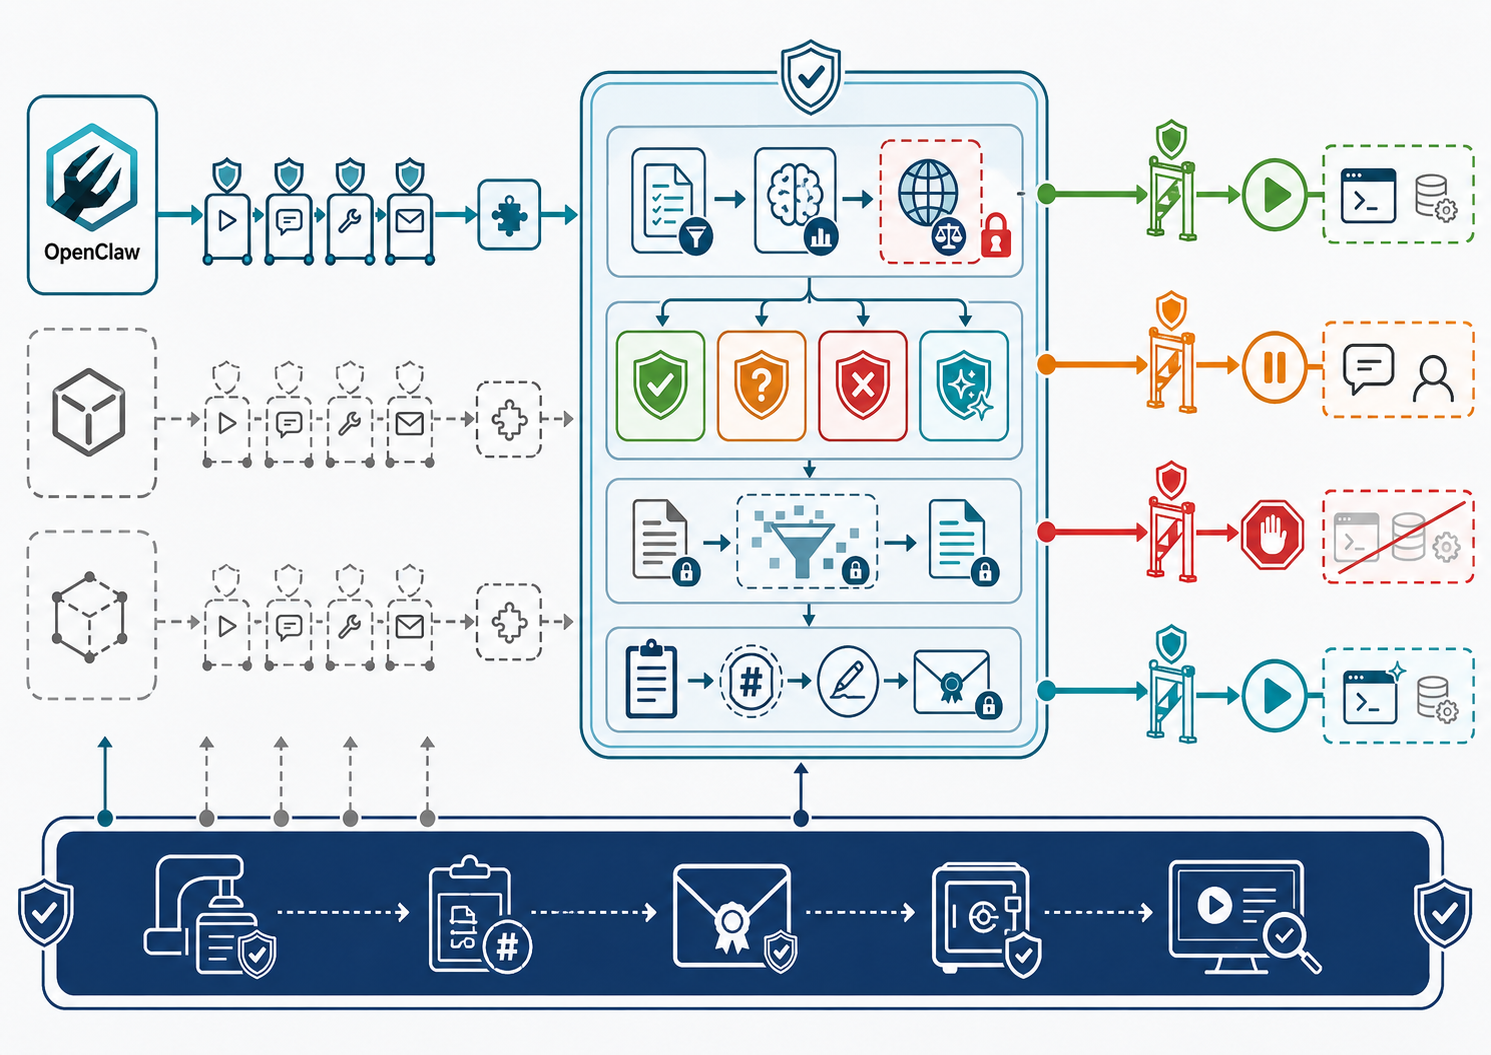
\includegraphics[width=\linewidth]{figures/page_33.png}
\end{center}

\subsection{结语}

灵鉴Agentscope 以三级级联判定、OpenClaw 四点强制和 300 条签名证据，交付\textbf{可复用、可执行、可审计、可重放}的智能体运行时安全中间件。
